\section{Arithmetic occurrence events and their prediction}\label{sec:events}
By \cref{thm:R3T1a} the realised geometry changes only when $D$ changes. This section separates the arithmetic bookkeeping (carries, plateaus) from the occurrence events, and proves an exact sieve that predicts the next event from the current state.

\subsection{Plateaus, carries and silent carries}
\begin{proposition}[plateau theorem]\label{prop:BT10}
Let $x=a/b$ with $D(x)\ne\emptyset$ and let $\delta=L^2/G$. Along any maximal run of steps on which $D$ is unchanged, $x_{n+j}=x_n+j\delta$: a plateau is an arithmetic progression with difference $\delta=L(x)^2/G(x)$.
\end{proposition}
\prov{CW-0392}{B-T10}{MIXED}{SPLIT}
\begin{proof}
If $D$ is unchanged then $L$ and $G$ are unchanged and $C(x)=x+L^2/G$ by definition. \qedhere
\end{proof}
\begin{example}[the plateau of $1369/9$; finite-exact]\label{ex:plateau}
$x_0=37^2/9$ has $D=\{37\}$, $L=37$, $G=36$, $\delta=1369/36$. The plateau has length $140$ and ends at $x_{140}=1369\cdot144/36=5476=4\cdot37^2$, an integer with $D\ni74$ (new element $74^2=5476$).
\end{example}
\begin{remark}
The source record also asserts the ruler-function pattern of the $2$-adic valuations on a plateau and the value $\pi(c+l)$ of a rank invariant. These parts are \emph{finite-exact} in the source and are \stat{cited}, not re-derived; the record is therefore split: the arithmetic-progression statement is proved above.
\end{remark}

\begin{definition}[carry, silent carry]\label{def:carry}
A step $x_n\to x_{n+1}$ is a \emph{carry} if the box changes (in either direction), i.e.\ $q_p(x_{n+1})\ne q_p(x_n)$ for some prime $p$ (a new active prime counts as a change from $q_p=0$), and an \emph{event} if $D(x_{n+1})\ne D(x_n)$. A carry that is not an event is \emph{silent}.
\end{definition}
\begin{theorem}[occurrence changes only at carries (regime I)]\label{thm:B2T8}
On a regime-I orbit with $m_n=t_n\sigma_n^2$, $D(m_n)=\{d\mid\sigma_n:d\ge2\}$ is non-decreasing; it changes exactly at the steps with $u_n>1$ (the carries of \cref{thm:B2T6}), and at such a step the number of new elements is $\tau(\sigma_nu_n)-\tau(\sigma_n)$. In particular, for $u=2$ and $\sigma=2^a\mu$ with $\mu$ odd the count is $\tau(\mu)$.
\end{theorem}
\prov{CW-0402}{B2-T8}{PROVED}{FULL}
\begin{proof}
$D(m)=\{d\mid\sigma:d\ge2\}$, so $|D|=\tau(\sigma)-1$ and $\sigma_{n+1}=\sigma_nu_n$ by \cref{thm:B2T6}; $D$ changes iff $u_n>1$. If $u=2$ and $\sigma=2^a\mu$, then $\tau(2\sigma)-\tau(\sigma)=(a+2)\tau(\mu)-(a+1)\tau(\mu)=\tau(\mu)$. \qedhere
\end{proof}
\begin{theorem}[constancy between events; silent carries]\label{thm:R3T6}
Along any orbit the realised complexes $\Kaxis(x_n)$, $\Kmove(x_n)$ (with boundaries, components and homology) are constant on every run of steps without an event, even through carries. Silent carries occur: the box can change while $D$ is fixed (\cref{fig:carries}).
\end{theorem}
\prov{CW-0421}{R3-T6}{MIXED}{SPLIT}
\begin{proof}
Constancy is \cref{thm:R3T1a}: the realised complexes are functions of $D$. A silent carry is exhibited by the $G=11$ tower: for $x_n=(j+1)S_0^2/11$, $S_0=2^23^35^4$, the exponent $q_2(x_n)=\lfloor v_2(a_n)/2\rfloor$ follows the $2$-adic valuation of the factor $j+1$ and equals $3$ instead of $2$ at $n=3,7,11,15$ (returning at $n=4,8,12,16$), while $D$ changes only at $n=8$ and $n=16$, where $q_3$ rises (\cref{fig:carries}). \qedhere
\end{proof}
\begin{remark}
The \stat{finite-exact} part of the source record, the table of Betti vectors of the $\ell=11$ tower for $k\le11$, is superseded in this paper by the longer exact table to $k=140$ of \cref{sec:towertop}; no claim is made beyond the computed range.
\end{remark}
\begin{figure}[tbp]\centering
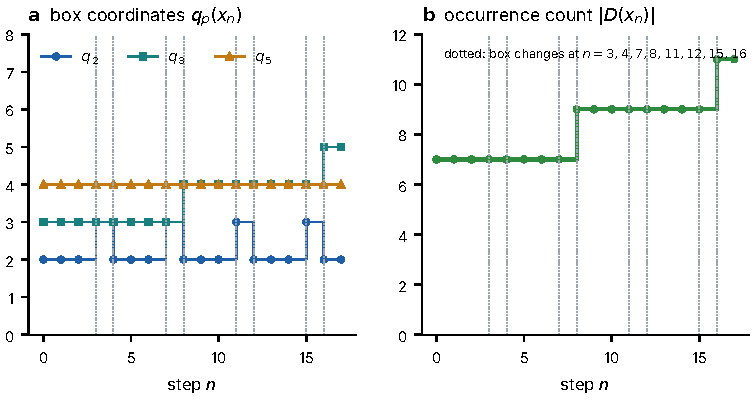
\includegraphics[width=\textwidth]{fig10_carries_vs_events}
\caption{\textbf{Carries versus events (finite-exact; illustrates \cref{thm:R3T6}).} Parameters: $G=11$ tower, $S_0=2^2\,3^3\,5^4$, $x_0=S_0^2/11$, steps $n=0..17$. (a) box coordinates $q_2,q_3,q_5$ of $x_n$ (a carry occurs wherever one of them changes; dotted lines mark the steps $n=3,4,7,8,11,12,15,16$). (b) occurrence count $|D(x_n)|$: constant except for its two jumps, at $n=8$ and $n=16$. Carries at $n=3,4,7,11,12,15$ are silent. The box coordinates are arithmetic data of the numerator; the count $|D|$ is the geometric (occurrence) datum. The range shown is the checked range.}\label{fig:carries}
\end{figure}

\subsection{The stage sieve}
Let $x=a/b$ be a state with $D(x)\ne\emptyset$, $G=G(x)=bh$, $L=L(x)$, and put $Y_j=ah+jL^2$. For a plateau starting at $x$ (so that $L,G$ are fixed), $x_{j}:=C^j(x)=Y_j/G$ as long as $D$ is unchanged; $Y_j/G$ need not be reduced.
\begin{definition}[sieve modulus]\label{def:Q}
For an integer $d\ge2$ put $r(d)=G/\gcd(d-1,G)$ and
\[
Q(d)=\lcm\Big(r(d),\ \prod_{p\mid d}p^{\,2v_p(d)+v_p(G)}\Big).
\]
\end{definition}
\begin{theorem}[stage sieve]\label{thm:sieve}
For every $j\ge0$ and every integer $d\ge2$: $d\in D(Y_j/G)\iff Q(d)\mid Y_j$.
\end{theorem}
\prov{CW-0437}{A5-T2.1}{PROVED}{FULL}
\begin{proof}
Let $g=\gcd(Y_j,G)$, $N=Y_j/g$, $B=G/g$, so $Y_j/G=N/B$ is reduced and $d\in D$ iff $d^2\mid N$ and $B\mid d-1$.

\emph{($\Rightarrow$)} Suppose $d^2\mid N$ and let $p\mid d$, $v=v_p(d)$. If $p\mid G$ then $v_p(g)=v_p(G)$: otherwise $v_p(g)=v_p(Y_j)$ and $v_p(N)=0<2v$. If $p\nmid G$, $v_p(g)=0=v_p(G)$. In both cases $v_p(Y_j)\ge2v+v_p(G)$. Next $B\mid d-1$ means $B\mid e:=\gcd(d-1,G)$, i.e.\ $G\mid eg$, i.e.\ $r(d)=G/e\mid g\mid Y_j$.

\emph{($\Leftarrow$)} If $Q(d)\mid Y_j$ then $r(d)\mid\gcd(Y_j,G)=g$, hence $B\mid d-1$ by the same equivalence. For $p\mid d$: $v_p(Y_j)\ge2v+v_p(G)$; if $p\mid G$ then $v_p(g)=v_p(G)$ and $v_p(N)=v_p(Y_j)-v_p(G)\ge2v$; if $p\nmid G$, $v_p(N)=v_p(Y_j)\ge2v$. So $d^2\mid N$. \qedhere
\end{proof}
\begin{corollary}[first-event law]\label{cor:event}
Let $\tau_D$ be the least $j\ge1$ such that some $d\notin D(x)$ satisfies $Q(d)\mid Y_j$ (equivalently $L^2j\equiv-ah\pmod{Q(d)}$). Then $D$ is unchanged for $0\le j<\tau_D$, the plateau has length $\tau_D$ and $D(x_{\tau_D})=\{d\ge2:Q(d)\mid Y_{\tau_D}\}\supsetneq D(x)$. Each candidate contributes one linear congruence, solvable iff $\gcd(L^2,Q(d))\mid ah$, with least positive solution found modulo $Q(d)/\gcd(L^2,Q(d))$.
\end{corollary}
\prov{CW-0438}{A5-T2.2}{PROVED}{FULL}
\begin{proof}
By \cref{thm:sieve}, $D(x_j)$ is the set of $d$ with $Q(d)\mid Y_j$ as long as $L,G$ are unchanged, i.e.\ until the first $j$ at which the set is larger than $D(x)$ (it always contains $D(x)$ by \cref{lem:M}). The condition $Q(d)\mid ah+jL^2$ is the stated congruence. \qedhere
\end{proof}
\begin{corollary}[events never stop]\label{cor:never}
For every state with $D\ne\emptyset$, $\tau_D<\infty$. Hence along every orbit with $D(x_0)\ne\emptyset$ there are infinitely many events and $|D(x_n)|\to\infty$.
\end{corollary}
\prov{CW-0439}{A5-T2.3}{PROVED}{FULL}
\begin{proof}
Choose a prime $p\nmid aGL$. Then $p\notin D(x)$ (since $p^2\nmid a$) and $Q(p)=r(p)p^2$ with $r(p)\mid G$ prime to $p$. The congruence $L^2j\equiv-ah\pmod{Q(p)}$ is solvable: $\gcd(L,G)=1$ (\cref{lem:basic}) and $p\nmid L$, so $L^2$ is invertible modulo $Q(p)$. Thus $\tau_D\le Q(p)<\infty$. After the event $D$ is again non-empty and strictly larger; iterate. \qedhere
\end{proof}
\Cref{fig:firstevent} illustrates the congruence for the first event.
\begin{figure}[tbp]\centering
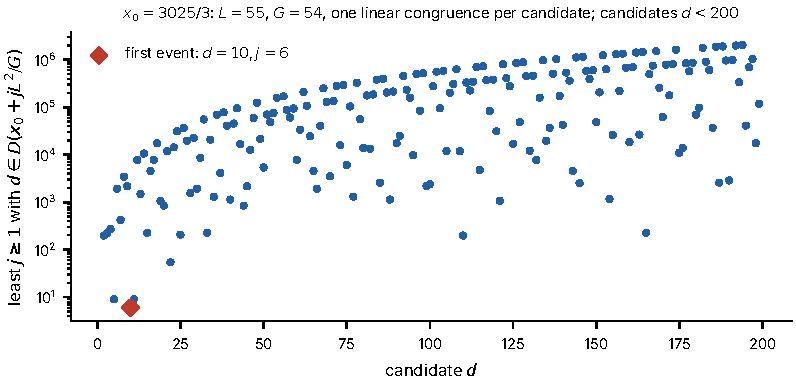
\includegraphics[width=\textwidth]{fig11_first_event}
\caption{\textbf{One linear congruence per candidate (exact computation; \cref{cor:event}).} $x_0=3025/3$: $a=3025$, $b=3$, $G=54$, $h=18$, $L=55$. Each point is a candidate $d<200$, $d\notin D$, for which the congruence is solvable, plotted at its least solution $j$. The minimum is $j=6$, attained at $d=10$ (diamond): the first event is at step $6$ and creates $10$. Finite-exact illustration, $d<200$ only; the law itself quantifies over all $d$.}\label{fig:firstevent}
\end{figure}

\subsection{Agreement with direct simulation}
\begin{remark}[finite-exact verification]\label{rem:nextevent}
The first-event law was tested against direct iteration of $C$ on $49$ states (orbits with $\tau_D\le200$ and the congruence search restricted to $\sqrt{ah+\tau L^2}\le30000$): the predicted step, and the full new set $\{d:Q(d)\mid Y_{\tau}\}$, agreed in all $49$ cases. A graph-level predictor (\cref{sec:prediction}) agreed on $175$ further events. Both are \stat{finite-exact} (\cref{fig:prediction}); no inherited suite was re-run.
\end{remark}
\begin{figure}[tbp]\centering
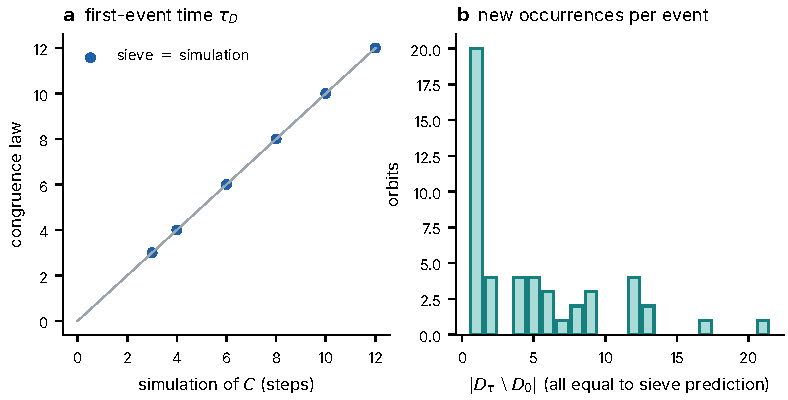
\includegraphics[width=\textwidth]{fig12_prediction}
\caption{\textbf{Prediction against reconstruction (finite-exact; $49$ states).} (a) first-event time from the congruence law versus the first event found by iterating $C$ (all points on the diagonal). (b) number of new occurrences per event; each count equals the sieve prediction. Orbits with $\tau_D\le200$ only; nothing outside this range is plotted or claimed.}\label{fig:prediction}
\end{figure}
